\documentclass[11pt,twoside]{article}
\usepackage{graphicx} % Required for inserting images
\usepackage[utf8]{inputenc}
\usepackage[T1]{fontenc}
\usepackage[french]{babel}
\usepackage{float}
\usepackage[
    left=3.18cm,
    right=3.18cm,
    top=2.54cm,
    bottom=2.54cm
]{geometry}
\usepackage{fancyhdr}


\pagestyle{fancy}

\fancyhf{} % clear all headers and footers

\fancyfoot[RO]{\thepage} % Right side on Odd pages
\fancyfoot[LE]{\thepage} % Left side on Even pages
\renewcommand{\headrulewidth}{0pt}
\renewcommand{\footrulewidth}{0pt}

\usepackage{setspace}
\setstretch{1.15}

\usepackage{amsmath} % for \numberwithin
\numberwithin{figure}{section}

\usepackage{caption}
\captionsetup{labelsep=colon,labelfont={footnotesize,bf},textfont={footnotesize,normalfont}}
\usepackage{hyperref}
\usepackage{cleveref}
\crefname{figure}{figure}{figures}
\Crefname{figure}{Figure}{Figures}


\usepackage{booktabs} % Add this to your preamble

\begin{document}

% Section 1
\begin{titlepage}
\pagenumbering{roman}
\begin{flushright}
\textbf{Charles Bouthilier (536842818)}\\
\textbf{Zied Gharbi (536961413)}\\
\textbf{Poste 05}\\
\end{flushright}
\centering

\vspace*{1cm}

{\Large \textbf{Laboratoire sur la mesure de l'accélération gravitationnelle}} \\[0.5cm]
{\large Rapport du travail pratique 8, cours GMC-3006} \\[0.5cm]

\vfill

\begin{figure} [H]
    \centering
    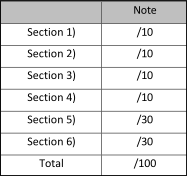
\includegraphics[width=0.40\linewidth]{imags/grid.png}
\end{figure}

\vfill

Faculté des sciences et de génie \\ [0.25cm]
Génie mécanique \\ [0.25cm]
Université Laval

\vspace{0.5cm}

1 avril 2026

\end{titlepage}

\tableofcontents
\newpage


%Section 2
\newpage
\pagenumbering{arabic}
\thispagestyle{empty}
\section{Tableaux des données expérimentales et résultats}

\begin{table}[h]
\centering
\caption{Tableau des données expérimentales de la chute libre.}
\label{tab:donnees_chute}
\begin{tabular}{@{}lccc@{}}
\toprule
\multicolumn{4}{c}{\textbf{Mesure des hauteurs}} \\ \midrule
$z_1$ [mm] & \multicolumn{3}{c}{0.00} \\
$z_2$ [mm] & \multicolumn{3}{c}{115.71} \\
$z_3$ [mm] & \multicolumn{3}{c}{227.05} \\ \midrule
\multicolumn{4}{c}{\textbf{Mesure des temps}} \\ \midrule
 & \textbf{1 kHz} & \textbf{10 kHz} & \textbf{75 kHz} \\ \midrule
$t_1$ [sec] & 0.249 & 0.2495 & 0.249964\\
$t_2$ [sec] & 0.293 & 0.2932 & 0.293727\\
$t_3$ [sec] & 0.329 & 0.3298 & 0.330251\\
\bottomrule
\end{tabular}
\end{table}

\begin{table}[h]
\centering
\caption{Tableau des données expérimentales du pendule.}
\label{tab:donnees_pendule}
\begin{tabular}{@{}lccc@{}}
\toprule
\multicolumn{2}{c}{\textbf{Mesure des Longueurs}} \\ \midrule
$L_{CP}$ [mm] & 830.25 \\
$L_{m}$ [mm] & 19.22 \\
\multicolumn{2}{c}{\textbf{Mesure des temps}} \\ \midrule
$t_i$ [sec] & 0.45944 \\
$t_f$ [sec] & 2.29664 \\
\bottomrule
\end{tabular}
\end{table}

\begin{table}[H]
    \centering
    \caption{Résultat de la mesure de $g$ et de son incertitude selon 4 types de tests}
    \label{tab:g_incertitude}
    \begin{tabular}{|c|c|c|c|c|}
        \hline
        Type de test & $u_g$ calculé & $g$ mesuré & $g_{\min} = g_{\text{mesuré}} - u_{g}$ & $g_{\max} = g_{\text{mesuré}} + u_{g}$\\
        \hline
        \multicolumn{5}{|c|}{[$m/s^{2}$]} \\
        \hline
        \textbf{Chute à 1kHz} & & 11.575 & &  \\
        \hline
        \textbf{Chute à 10kHz} & & 9.819 & & \\
        \hline
        \textbf{Chute à 75 kHz} & & 10.074 & & \\
        \hline
        \textbf{Pendule}& & 9.823 & & \\
        \hline
    \end{tabular}
\end{table}
%Section 3
\newpage
\section{Programmes utilisés}
\thispagestyle{empty}

\subsection{Prise de données}
\subsection{Analyse des données}


%Section 5
\newpage{}
\section{Analyse et questions}
\thispagestyle{empty}

\subsection{La valeur théorique est-elle dans l'interval de confiance?}

\subsection{Quels sont les paramètres qui ont le plus grand impact sur l'incertitude?}

\newpage{}
\section{programme d'analyse d'incertitude}
\thispagestyle{empty}


%Bibliographie
\newpage
\thispagestyle{empty}
\begin{thebibliography}{9}

\bibitem{Lemay2017}
Lemay, Jean.
(2017).
\textit{Mesure, mécatronique et traitements de données}.
Éditions JFD inc.


\end{thebibliography}

\end{document}
